% !TeX root = ../main.tex
% %%%%%%%%%%%%%%%%%%%%%%%%%%%%%%%%%%%%%%%%%%%%%%%%%%%%%%%%%%%%%%%%%%%%%%%%%%%%%%
% Introduction
\chapter{Introduction}
\label{chap:introduction}

\alcides{Começas com uma frase sem dar suporte. Precisa de uma frase inicial a dar exemplos de robots e como são úteis. Nem toda a gente concordaria}

Robotics already have a great impact in our current society so, 
the quality of software used by robots should be of extreme importance for us.
Robot software as well as the techniques used to test their quality are 
very specific to the field \todo{field-specific} and different from the techniques employed in traditional Software Engineering.
Automatic tests are barely used in robotics due to multiple factors: \todo{enumerate what factors. Don't leave the reader hanging.}



\todo{O parágrafo seguinte tenta avançar muito na ideia, sem estabelecer as bases.}
The intention is then to create a tool that will promote the safe 
and reliable execution of automatic tests.
This tool will contemplate both a descriptive high-level language 
that should capture certain properties of a robot and a way to create test scenarios.
\todo{Alternative suggestion:
The goal of this thesis is to overcome the challenges of automated testing in robotics, by providing developers with an usable alternative that allows to detect bugs with less effort through simulation.}

% ------------------------------------------------------------------------------
% Motivation
\section{Motivation}
\label{sec:motivation}

\todo{Today}, robots are vastly used industrially (medicine, agriculture, etc.) 
or leisurely (contests, personal use, etc.).
The tendency is for robot usage to keep growing at a global level.
Robot tasks tend to be repetitive and rather specific.
\todo{Therefore,} Robot software also tends to be quite different from conventional software.
The Cyber-Physical systems of robots are non-deterministic and unreliable, mainly because robots interact directly with their environment.
A sensor can return imprecise values since the environment itself can be very hard to predict.
As a result, verifying whether a task or movement is correct is hard for a robot to conceive.

\par

Current practices on testing robot software are common among developers, including field testing, simulation testing, logs checking, among others.
The common denominator among these is that they require a human to analyze the behavior of the robot to determine whether the behavior is correct. If there was a tool that could make this decision, automated tests could be used more widely in robot systems.
However, that is not the case as automatic tests are hardly used. Opening this door would mean an improvement 
in the quality of current and future robot software.


\section{Problem Statement}
\label{sec:problem}

There are multiple challenges in robot testing: cost, 
complexity, hardware integration, among others.
When planning on how to test a robot there are tradeoffs among all the challenges.
While simulation-based tests are a promising approach for automation 
there is still distrust in the precision and validity of the results.
This means that, despite being dangerous and sometimes expensive, real-life 
robot testing is still the main choice.

Both in real-world testing or in simulations, 
human supervising will most likely still be necessary.
This is because identifying if a robot fulfills an expected 
behavior is really hard for the robot itself.
For this reason, automatic tests in the robotics field are 
hardly reliable and hard to implement.
The resulting product is a lack of quality in the software 
across projects~\cite{TestRob}.

\todo{Li o parágrafo, mas fiquei sem saber qual era o problema. É importante ter uma frase no final a resumir de forma simples o problema.}

% ------------------------------------------------------------------------------
% Objectives
\section{Objectives}
\label{sec:objectives}

This work has the objective of showing the potencial of automatic 
tests in robotics and of simplifying their execution.

\todo{A linha desta secção perde-me.}

\todo{Propomos que os developers descrevam o cenário a testar usando uma linguagem de alto nível.}
\todo{A partir da descrição dessa linguagem, iremos detectar e instrumentar os componentes do robot relevantes.}
\todo{A monitorização da execução ou, em alternativa, uma análise aos logs do robot irão detectar desvios ao comportamento normal do robot. }


With this in mind, we propose a mechanism that monitors a subset of the components of the robot during or after a test execution.
These components aren't arbitrary but defined by the help of a descriptive high-level language.
The objective of the language is to describe a robot property in a simple and intuitive way.
This language will need to be supported by a compiler. 
The compiler should translate the language to a monitoring mechanism.
In this way, if a robot doesn't follow the properties defined by the language 
during a test, the compiler will infer that the robot behavior isn't correct. \todo{Acho que o compilador não vai detectar estas!}

\par

\todo{Este parágrafo não encaixa bem aqui. O ROS deve ir para o capítulo Background e o Gazebo para related work.}
The Robot Operating System (ROS) is a collection of libraries and tools that help 
build robot software. ROS is the most widely used tool for writing robot software.
Robot simulation is an essential tool for testing. Gazebo offers the ability 
to simulate populations of robots in complex environments.
This being said, the final scheme of the tool that will accomplish the objective 
should look something like the below image.

\begin{figure}[h!]
    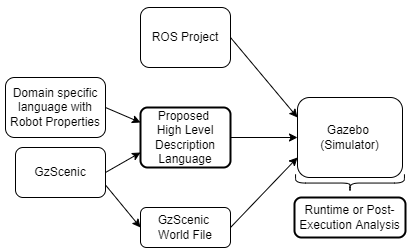
\includegraphics{images/intro_diag.png}
    \caption{Tool for monitoring robot properties.}
    \label{fig:intro_objectives}
\end{figure}
\todo{esta imagem tem de ser melhorada bastante.}

\section{Contributions}
\label{sec:contributions}

The expected contributions of this thesis are below enumerated.

\begin{enumerate}
    \item Definition of a descriptive high-level language to specify robots properties.
    \item Implementation of compiler for the language that can be used for monitoring.
    \item Evaluation of the expressive capability of the solution in real-world examples.
\end{enumerate}

% ------------------------------------------------------------------------------
% Structure of the document
\section{Structure of the document}
\label{sec:structure}

The document is organized as follows:

\begin{itemize}
    \item Section 1...
    \item Section 2...
    \item Section 3...
\end{itemize}

